\begin{margintable}
\scalebox{1.1}{
\begin{tabular}{cc}
	\raisebox{-.5in}{
	\begin{tabular}[b]{r|l} 
	$x$ & $f(x)$ \\ 
	\hline $-0.9$ & $2.9$ \\ 
	$-0.99$ & $2.99$ \\ 
	$-0.999$ & $2.999$ \\ 
	$-0.9999$ & $2.9999$ \\ 
	$-1.1$ & $3.1$ \\ 
	$-1.01$ & $3.01$ \\ 
	$-1.001$ & $3.001$ \\ 
	$-1.0001$ & $3.0001$ \\ 
	\end{tabular} } &	
	\raisebox{-.5in}{
	\begin{tabular}[b]{r|l} 
	$x$ & $f(x)$ \\ 
	\hline $-1.9$ & $3.9$ \\ 
	$-1.99$ & $3.99$ \\ 
	$-1.999$ & $3.999$ \\ 
	$-1.9999$ & $3.9999$ \\ 
	$-2.1$ & $4.1$ \\ 
	$-2.01$ & $4.01$ \\ 
	$-2.001$ & $4.001$ \\ 
	$-2.0001$ & $4.0001$ \\ 
	\end{tabular} }
\end{tabular}
} % end scalebox 
\caption{Function values near $-1$ and $-2$.} \label{T:1-1_Eg1}
\end{margintable}

\begin{marginfigure}
\margingraphics{figures/1_2_Ex1f.eps}
\caption{The graph of $f(x) = \frac{4-x^2}{x+2}$ near $-1$ and $-2$.}\label{fig:1-1_Eg1}
\end{marginfigure}

\begin{example} \label{Ex:1.1.Eg1}
Use both tables and graphical approaches to investigate and, if possible, estimate or determine the value of the limit for the following function at the specified values.  
\[ \ds f(x) = \frac{4-x^2}{x+2}; \quad a = -1, \ a = -2 \]

\solution We first construct tables of values near $a = -1$ and $a = -2$, see Table~\ref{T:1-1_Eg1}, along with a graph of $f$, see Figure~\ref{fig:1-1_Eg1}.  

From the left table, it appears that we can make $f$ as close as we want to $3$ by taking $x$ sufficiently close to $-1$, which suggests that $\ds \lim_{x \to -1} f(x) = 3$.	This is also consistent with the graph of $f$.  

From the right table, it appears that we can make $f$ as close as we want to $4$ by taking $x$ sufficiently close, but not equal since $f(-2)$ is not defined, to $-2$, which suggests that $\ds \lim_{x \to -4} f(x) = 4$.	Remember, limits ask, ``To where is the function going?'', not ``What is the value of the function?''  Again, this observation is  consistent with the graph of $f$.  

%Next we turn to the function $g$, and construct two tables and a graph.
%\begin{figure}[h]
%\centering
%\begin{tabular}{ccc}
%	\raisebox{-.05in}{\begin{tabular}[b]{r|l} $x$ & $g(x)$ \\ \hline 2.9 & 0.84864 \\ 2.99 & 0.86428 \\ 2.999 & 0.86585 \\ 2.9999 & 0.86601 \\ 3.1 & 0.88351 \\ 3.01 &  0.86777 \\ 3.001 & 0.86620 \\ 3.0001 &  0.86604 \\ \end{tabular} } &	
%	\raisebox{-.05in}{\begin{tabular}[b]{r|l} $x$ & $g(x)$ \\ \hline -0.1 & 0 \\ -0.01 & 0 \\ -0.001 & 0 \\ -0.0001 & 0 \\ 0.1 & 0 \\ 0.01 & 0 \\ 0.001 & 0 \\ 0.0001 & 0 \\ \end{tabular} } &
%	\hspace{0.25in} 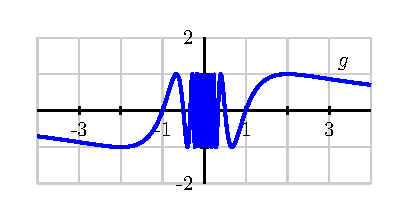
\includegraphics{figures/1_2_Ex1g.eps} 
%\end{tabular}
%\caption{Tables and graph for $\ds g(x) = \sin\left(\frac{\pi}{x}\right)$.} \label{F:1.2.Ex1g}
%\end{figure}

%First, as $x \to 3$, it appears from the data (and the graph) that the function is approaching approximately $0.866025$.  To be precise, we have to use the fact that $\frac{\pi}{x} \to \frac{\pi}{3}$, and thus we find that $g(x) = \sin(\frac{\pi}{x}) \to \sin(\frac{\pi}{3})$ as $x \to 3$.  The exact value of $\sin(\frac{\pi}{3})$ is $\frac{\sqrt{3}}{2}$, which is approximately 0.8660254038.  Thus, we see that
%$$\lim_{x \to 3} g(x) = \frac{\sqrt{3}}{2}.$$
%
%As $x \to 0$, we observe that $\frac{\pi}{x}$ does not behave in an elementary way.  When $x$ is positive and approaching zero, we are dividing by smaller and smaller positive values, and $\frac{\pi}{x}$ increases without bound.  When $x$ is negative and approaching zero, $\frac{\pi}{x}$ decreases without bound.  In this sense, as we get close to $x = 0$, the inputs to the sine function are growing rapidly, and this leads to wild oscillations in the graph of $g$.  It is an instructive exercise to plot the function $g(x) = \sin\left(\frac{\pi}{x}\right)$ with a graphing utility and then zoom in on $x = 0$.  Doing so shows that the function never settles down to a single value near the origin and suggests that $g$ does not have a limit at $x = 0$.

\end{example}